\documentclass[12pt]{article}
\usepackage{lingmacros}
\usepackage{tree-dvips}
\usepackage[utf8]{inputenc}
\usepackage[russian]{babel}
\usepackage{amsmath,amssymb}
\usepackage{multirow}
\usepackage{hyperref}
\usepackage{caption}
\usepackage{tabularx}
\usepackage{graphicx}

\begin{document}

\section*{Задачи}

\subsection*{Лесни}
\subsubsection*{Задача 1.1}
Да се докаже, че $\displaystyle\sum_{i=1}^{n} i = \frac{n(n+1)}{2}$
\subsubsection*{Задача 1.2}
Да се докаже, че $\displaystyle\sum_{i=1}^{n} \frac{1}{i(i+1)} = \frac{n}{n+1}$
\subsubsection*{Задача 1.3}
Да се докаже, че $\displaystyle\sum_{i=0}^{n} 2^i = 2^{n+1} - 1$
\subsubsection*{Задача 1.4}
Да се докаже, че $5^{2n + 1} + 2^{2n+1}$ се дели на $7$ за всяко $n \in \mathbb{N}$
\subsubsection*{Задача 1.5}
Да се докаже, че $f_{n+1} < \biggl( \frac{7}{4} \biggr)^n$, където $f_{n+1}$ е $(n+1)$-вото число на Фибоначи.
\subsubsection*{Задача 1.6}
Да се докаже, че за всяко цяло число $n \geq 2$ е в сила, че $\displaystyle\prod_{k=1}^n \biggl(1 - \frac{1}{\sqrt{k}}\biggr) < \frac{2}{n^2}$
\subsection*{Задача 1.7 - Задачи за самоподготовка по Дискретни структури - 2021/2022 - Добромир Кралчев}
Да се докаже, че $\frac{1}{n+1} + \frac{1}{n+2} + \frac{1}{n+3} + ... + \frac{1}{3n + 1} > 1$ за всяко $n \geq 1$
\subsection*{Задача 1.8 - Kenneth H. Rosen}
Да се докаже, че за всяко $n \in \mathbb{N}$
\begin{equation*}
    \displaystyle\sum_{k=1}^{2^n} \frac{1}{k} \leq 1 + n
\end{equation*}

\subsection*{По-забавни}
\subsubsection*{Задача 2.1}
Да се докаже, че $\displaystyle\sum_{X \subseteq \{ 1, 2, ..., n \}} \prod_{y \in X} y = (n+1)!$.
\subsubsection*{Задача 2.2}
Да се докаже, че сумата на първите $n$ нечетни числа е точен квадрат за всяко $n \in \mathbb{N}$.
\subsubsection*{Задача 2.3}
Да се докаже, $1 + \frac{1}{4} + \frac{1}{9} + ... + \frac{1}{n^2} < 2$ за всяко $n \in \mathbb{N}^+$.
\subsubsection*{Задача 2.4 - Записки на Ангел Димитриев}
Да се докаже, че всяко $n \in \mathbb{N}^+$ може да се представи като сума на \textbf{различни} степени на двойката.
\subsubsection*{Задача 2.5}
Да се докаже, че всяко естествено число $n \geq 2$ може да се представи като произведение на прости числа.
\subsubsection*{Задача 2.6}
Да се докаже, че всяка сума $n \geq 12$ може да се направи с банкноти от 4 и 5 лева.
\subsubsection*{Задача 2.7 - Kenneth H. Rosen}
Да се докаже, че всяка дъска с квадратчета с размери $2^n \times 2^n$ с едно квадратче премахнато може да се покрие с правоъгълни троминота(могат да се въртят).
\begin{figure}[!ht]
    \caption*{Правоъгълно тромино}
    \centering
    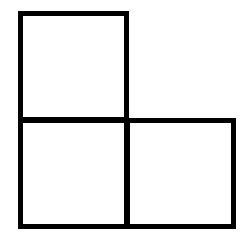
\includegraphics[height=1cm]{right-trominoe}
\end{figure}
    


\section*{Решения}

\end{document}